\section{Données de commande pour recentrer l'objectif de la caméra}

\begin{enumerate}
  \item \q{Ecrire une fonction qui retourne un quadruplet de booléenscontenant
          les données L+, L-, H+ ou H- indiquant si la nacelle doit être réorientée
          suivant la longueur ou la hauteur de l’image et suivant le sens.}

        \codeFromFileT{helpers/image.py}{section-05/q1-1.py}
        \codeFromFileT{helpers/image.py}{section-05/q1-2.py}
        J'obtiens alors :
        \codeFromFile{section-05/q1-3.txt}

        J'ai effectué en zoom sur la partie intéressante, on voit alors que le
        centre de la voiture est tout juste dans le rectangle vert,
        ce qui explique qu'il ne faille pas bouger la caméra.
        \begin{center}
          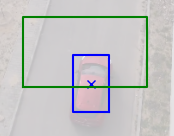
\includegraphics[scale=0.8]{section-05/q1-4.png}
        \end{center}
\end{enumerate}
